\documentclass[times, utf8, zavrsni, numeric]{fer}
\usepackage{booktabs}
\usepackage[hidelinks]{hyperref}
\usepackage{graphicx}

\setlength\parindent{24pt}
\newcommand{\matr}[1]{\mathbf{#1}}

\graphicspath{{"D:/fer/6. semestar/ZAVRAD/svm-sentiment-analysis/Thesis/Slike/"}}

\begin{document}

% TODO: Navedite broj rada.
\thesisnumber{000}

% TODO: Navedite naslov rada.
\title{Primjena stroja s potpornim vektorima za analizu sentimenta korisničkih recenzija}

% TODO: Navedite svoje ime i prezime.
\author{Dominik Stanojević}

\maketitle

% Ispis stranice s napomenom o umetanju izvornika rada. Uklonite naredbu \izvornik ako želite izbaciti tu stranicu.
\izvornik

% Dodavanje zahvale ili prazne stranice. Ako ne želite dodati zahvalu, naredbu ostavite radi prazne stranice.
\zahvala{Zahvaljujem se Donaldu E. Knuthu, Bogu računarske znanosti.}

\tableofcontents

\chapter{Uvod}

\par Klasifikacijski i regresijski problemi jedni su od najvažnijih problema strojnog učenja. 
Modeli poput linearne i logističke regresije pogodni su za jednostavnije probleme.
Zahvaljujući sve većoj dostupnosti podataka i povećanju procesorske moći današnjih računala,
pojavljuju se složeniji zadaci za koje navedene metode nisu efikasne.

\par Pojava složenijih zadataka rezultirala je i pojavom složenijih metoda koje mogu doskočiti 
istima. Modeli poput slučajnih šuma i modeli iz skupine dubokog učenja u mogućnosti su rješavati i složenije, 
nelinearne probleme.

\par Osim navedenih modela, još jedan model koji je sposoban efikasno obraditi nelinearne podatke 
je \textbf{stroj s potpornim vektorima} (engl. \textit{Support Vector Machine}).
Koristeći jezgreni trik, stroj s potpornim vektorima uspješno razdvaja linearno nerazdvojive podatke.
Iako su temeljne ideje modela predstavljene prije više od pola stoljeća, stroj s potpornim vektorima i danas je jedan od
najrobusnijih modela za klasifikaciju i regresiju.

\par Jedan od zanimljivih problema koji dobro prikazuje robusnost SVM-a je \textbf{analiza sentimenta}
(engl. \textit{Sentiment Analysis}).
Subjektivnost emocija, kontekst te velika količina podataka svakako predstavljaju izazove u rješavanju problema.
Koristeći SVM, uz uvjet kvalitetnog pretprocesiranja podataka, mogu se postići zavidni rezultati u polju analize sentimenta.

\par U radu je predstavljen model stroja s potpornim vektorima te problem analize sentimenta.
U drugom poglavlju bit će predstavljen pregled područja, povijest modela stroja s potpornim vektorima te problem analize sentimenta.
U trećem poglavlju detaljnije će se obraditi model SVM.
Bit će opisana motivacija i interpretacija modela.
Nadalje, detaljnije će se pojasniti algoritmi optimizacije modela.
U četvrtom poglavlju formalizirat će se problem analize sentimenta.
Prikazat će se postupak pretprocesiranja podataka koji će podatke pretvoriti u oblik razumljiv SVM-u.
U petom poglavlju, provest će se eksperiment analize korisničkih recenzija uporabom opisanih metoda.
Ukratko će se analizirati dobiveni rezultati.
Šesto poglavlje sadrži zaključak i ideje za daljnje istraživanje. 

\chapter{Pregled područja} \label{ppodrucja}
Započinje \cite{vapnik1963}

\chapter{Stroj s potpornim vektorima} \label{svm}
U ovom poglavlju bit će predstavljen model stroja s potpornim vektorima. 
U potpoglavlju \ref{hmargine} pojasnit će se ideja razdvajajuće hiperravnine.
Uz pomoć hiperravnine margine, u potpoglavlju \ref{ginter} iznijet će se geometrijska interpretacija modela.

\section{Razdvajajuća hiperravnina} \label{hmargine}
Interpretaciju modela stroja s potpornim vektorima potrebno je započeti s pojmom koji nije strogo vezan uz sam model.
Primjerice model logističke regresije, iako temeljen na vjerojatnosti, u konačnici pronalazi hiperravninu kojom može razdvojiti
podatke.

\par Neka je zadan prostor $\textit{X}$ dimenzije $n$.
Tada je \textbf{hiperravnina} definirana kao potprostor dimenzije $n-1$ unutar prostora $\textit{X}$.
Primjerice, u dvodimenzijskom prostoru hiperravnina predstavlja bilo koji pravac koji leži u ravnini. 
Analogno, pojam hiperravnine vrijedi i za prostore većih dimenzija. 

\par Za hiperravninu zadanom jednadžbom $f(x)=\beta_0 + \beta^Tx = 0$ vrijede sljedeća svojstva:
\begin{enumerate}
  \item Za svaku točku $T$ na hiperravnini vrijedi: $\beta_0 = -\beta^Tx$
  \item Normala zadana izrazom: $\mathbf{n} = \frac{\beta}{\|\beta\|}$
  \item Udaljenost točke $P$ od hiperravnine iznosi: $d = \frac{f(x)}{\|\beta\|}$
\end{enumerate}

\par Osim pojma hiperravnine, potrebno je definirati i pojam binarnog klasifikatora. 
Neka je upravo prostor $\textit{X}$ ulazni prostor koji definira potpun skup primjera. 
Svakom primjeru $\matr{x}=(x_1,x_2,\dots,x_n)$ pridružena je oznaka razreda $y$. 
Neka $y$ poprima vrijednosti iz skupa $\textit{C}$. 
Ako se klasificiraju podaci koji su podijeljeni u dva razreda, tj. $\left\vert{C}\right\vert=2$, tada se govori o binarnoj klasifikaciji. 
\textbf{Binarni klasifikator} je klasifikator koji može provesti binarnu klasifikaciju. 

\par Hiperravnine same po sebi nisu pretjerano interesantne. 
No, za klasifikaciju interesantan je određen podskup margina. 
Hiperravnina koja razdvaja dva razreda podataka naziva se \textbf{razdvajajuća hiperravnina.}

\begin{figure}
\centering
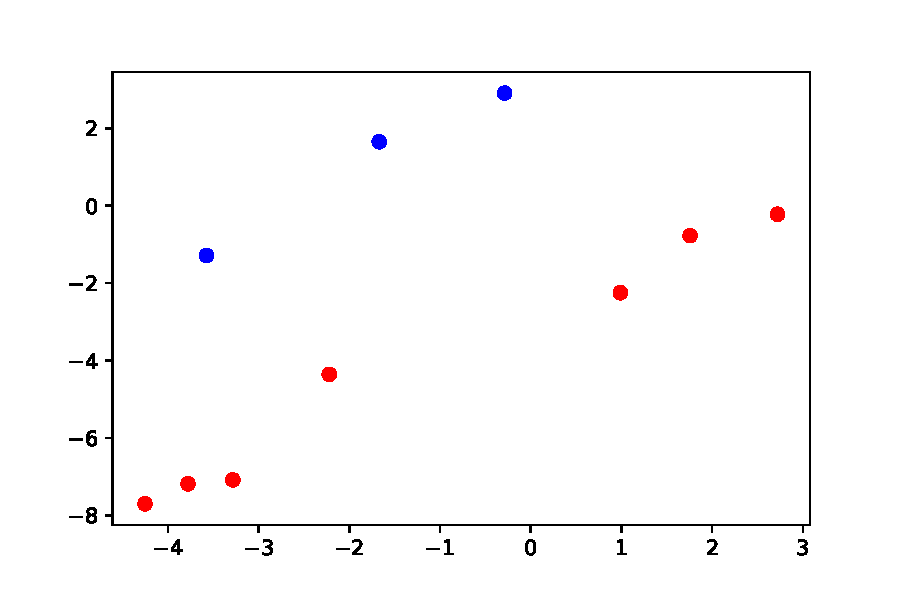
\includegraphics{tocke.pdf}
\caption{Razdvajajuće hiperravnine}
\label{fig:hrav}
\end{figure}

Na slici \ref{fig:hrav} prikazani su linearno razdvojivi podaci. 
Također, prikazane su i dvije razdvajajuće hiperravnine. 
Valja primijetiti kako je moguće konstruirati beskonačno mnogo razdvajajućih hiperravnina.

\par 



\section{Geometrijska interpretacija modela} \label{ginter}

\chapter{Analiza sentimenta} \label{sentiment}

\chapter{Eksperiment} \label{eksperiment}

\chapter{Zaključak} \label{zakljucak}
Zaključak.

\bibliography{literatura}
\bibliographystyle{fer}

\begin{sazetak}
Sažetak na hrvatskom jeziku.

\kljucnerijeci{Ključne riječi, odvojene zarezima.}
\end{sazetak}

% TODO: Navedite naslov na engleskom jeziku.
\engtitle{Title}
\begin{abstract}
Abstract.

\keywords{Keywords.}
\end{abstract}

\end{document}
